\section{Testing}

\subsection{\code{stacscheck} tests}

The project passes all \code{stacscheck} tests, as can be seen in the screenshot below which depicts the final few lines of the output.

\begin{center}
    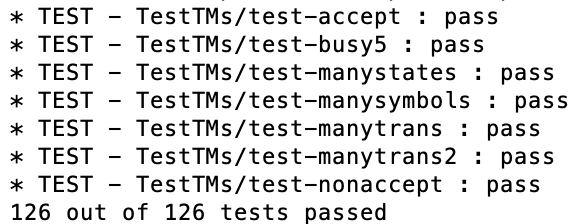
\includegraphics[width=0.5\textwidth]{images/screenshots/stacscheck.png}
\end{center}

\subsection{Custom automated tests}

To automate the testing of the Turing machines that were not covered by \code{stacscheck}, a custom testing tool was developed. This tests the $M_\text{binaryunary}$, $M_\text{subword}$, and $M_\text{subword\_fast}$ machines. The tool allows two types of tests: tests that verify that the machine correctly accepts and rejects, and tests that verify that the tape output is correct. 

To execute these tests, run \code{make tests} from the \code{src/} folder. The screenshot below shows that the Turing machines passed all tests.

\begin{center}
    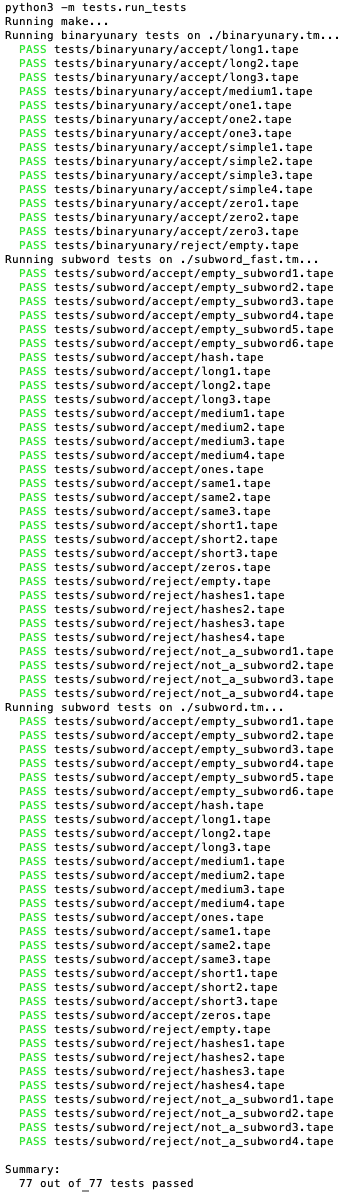
\includegraphics[height=\textheight]{images/screenshots/tests.png}
\end{center}